\documentclass[11pt]{article}

\usepackage{graphicx}
\usepackage{booktabs}
\usepackage{amsmath}
\usepackage{geometry}
\usepackage{hyperref}

\geometry{margin=1in}

\title{Predicting Diagnostic Outcomes Using Machine Learning}
\author{Saif Ur Rehman, Laura Valentina Sierra Pena, Ainur Smailova}
\date{\today}

\begin{document}

\maketitle

\section{Problem Formulation}

The objective of this study is to predict patient diagnostic outcomes using demographic and clinical variables. The dataset contains measurements related to sleep quality, fatigue severity, stress levels, and behavioural indicators. The target variable \textit{diagnosis} contains three categories: \textit{Depression}, \textit{CI}, and \textit{Both}. Consequently, the task is formulated as a supervised multiclass classification problem.

The dataset initially contained 670 observations and 19 variables. The goal is to determine whether the available demographic and clinical variables can accurately predict patient diagnosis.

\section{Data Analysis and Feature Selection}

Initial data exploration confirmed that the dataset contains no missing values and no duplicate observations. The dataset size is relatively small to moderate, making classical machine learning models more appropriate than deep learning approaches.

Inspection of the dataset revealed that the \textit{id} variable represents a unique patient identifier and therefore provides no predictive value. Additionally, the \textit{country} variable was constant across all observations and was removed from the dataset.

A statistical summary of the numerical variables revealed that the variable \textit{depression\_phq9\_score} contained a value of 99, which lies outside the valid clinical range (0--27) for the PHQ-9 depression scale. This observation was removed, resulting in a dataset containing 669 observations.

Several visualisation techniques were used to analyse the dataset. Histograms and violin plots were generated to examine distributional properties such as shape, symmetry, and density concentration. Most variables displayed smooth bounded distributions across their scales.

Boxplots were used to identify potential outliers. Although some values were detected outside the interquartile range for \textit{fatigue\_severity\_scale\_score} and \textit{depression\_phq9\_score}, these observations remained within clinically valid ranges and were therefore retained.

Scatterplots were used to investigate relationships between numerical variables. For example, the relationship between stress level and fatigue severity showed that fatigue severity tends to be higher for the \textit{CI} and \textit{Both} diagnostic groups, while stress levels were distributed across all categories.

Class distribution analysis revealed moderate class imbalance, with the \textit{Both} category containing fewer observations than the other classes. To ensure reliable evaluation, stratified sampling was adopted in the experimental protocol.

\subsection{Correlation and Redundancy Analysis}

A Pearson correlation heatmap was generated to examine relationships among numerical variables. A very strong correlation ($r=0.97$) was observed between \textit{sleep\_quality\_index} and \textit{deep\_sleep\_quality\_index}. Since highly correlated variables introduce redundancy and may negatively affect linear models, further analysis was performed.

Point plots and one-way ANOVA tests were conducted to examine whether these variables differed significantly across diagnostic groups. Neither variable showed statistically significant differences across classes. However, \textit{sleep\_quality\_index} demonstrated slightly stronger group separation and was therefore retained while \textit{deep\_sleep\_quality\_index} was removed.

\subsection{Categorical Association Analysis}

Cramér's V statistics were computed to evaluate associations between categorical variables and the target variable. The variable \textit{pem\_present} showed perfect association ($V=1.0$) with the target variable. Examination of the contingency table revealed that this variable deterministically partitioned the diagnostic classes. This represents target leakage and would artificially inflate model performance.

Therefore, \textit{pem\_present} was removed from the dataset.

After these preprocessing steps, the remaining features showed weak correlations and were considered suitable for modelling.

\section{Experimental Protocol}

To ensure reliable model evaluation, the dataset was divided into training and testing subsets using an 80/20 stratified train--test split. Stratification preserves class distribution across both subsets.

Model selection and hyperparameter tuning were performed using stratified 5-fold cross-validation on the training set. Macro F1-score was selected as the primary evaluation metric because it provides balanced performance across all classes and is robust to moderate class imbalance.

All preprocessing steps, including categorical encoding and feature scaling, were implemented within a machine learning pipeline to prevent data leakage during cross-validation.

\section{Machine Learning Methods}

Three classification algorithms discussed during lectures were selected for comparison:

\begin{itemize}
\item Logistic Regression
\item k-Nearest Neighbours (KNN)
\item Random Forest
\end{itemize}

These models represent different machine learning paradigms.

Logistic Regression is a linear classifier that models the relationship between predictors and the probability of each class. It provides a strong baseline model and assumes approximately linear relationships between features and the target.

KNN is a distance-based instance learning algorithm that classifies observations based on the labels of neighbouring data points in the feature space. It captures local similarity patterns without assuming a predefined functional form.

Random Forest is an ensemble tree-based model that combines multiple decision trees to capture nonlinear relationships and feature interactions. Ensemble methods such as Random Forest often perform well on structured tabular datasets.

\section{Hyperparameter Search}

Hyperparameter tuning was performed using grid search within stratified 5-fold cross-validation. Table~\ref{tab:hyperparameters} summarises the search spaces and best configurations obtained during model selection.

\begin{table}[h]
\centering
\resizebox{\textwidth}{!}{
\begin{tabular}{lccc}
\toprule
Model & Hyperparameter Grid & Best Hyperparameters & CV Macro F1 \\
\midrule
Logistic Regression & $C \in \{0.1,1,10\}$ & $C = 10$ & 0.774 \\
kNN & $k \in \{3,5,7,9,11\}$ & $k = 11$ & 0.548 \\
Random Forest & $n_{trees} \in \{200,500\}$, $depth \in \{None,10,20\}$ & $n_{trees}=500$, $depth=10$ & 0.947 \\
\bottomrule
\end{tabular}
}
\caption{Hyperparameter tuning results using grid search with stratified 5-fold cross-validation}
\label{tab:hyperparameters}
\end{table}

Random Forest achieved the highest cross-validation Macro F1-score. This indicates that nonlinear relationships and interactions between variables play an important role in predicting diagnostic outcomes.

\section{Model Comparison}

Table~\ref{tab:modelcomparison} summarises the performance of the evaluated models.

\begin{table}[h]
\centering
\begin{tabular}{lc}
\toprule
Model & Cross-Validated Macro F1 Score \\
\midrule
Logistic Regression & 0.774 \\
kNN & 0.548 \\
Random Forest & 0.947 \\
\bottomrule
\end{tabular}
\caption{Cross-validated performance comparison}
\label{tab:modelcomparison}
\end{table}

Random Forest significantly outperformed the other models. Logistic Regression achieved moderate performance, indicating that some linear structure exists in the dataset. In contrast, KNN performed substantially worse, suggesting that local neighbourhood similarity alone is insufficient to capture the complex patterns in the data.

\section{Final Model Evaluation}

The Random Forest model with the best hyperparameters ($n\_estimators=500$, $max\_depth=10$) was evaluated on the unseen test set.

The model achieved an accuracy of approximately 0.96 and a Macro F1-score of approximately 0.95, indicating strong predictive performance across all diagnostic categories.

The confusion matrix indicates that the \textit{CI} category was classified with perfect accuracy. The \textit{Depression} class also achieved high recall and precision. A small number of \textit{Both} cases were misclassified as \textit{Depression}, suggesting some overlap between these two diagnostic groups.

\begin{figure}[h]
\centering
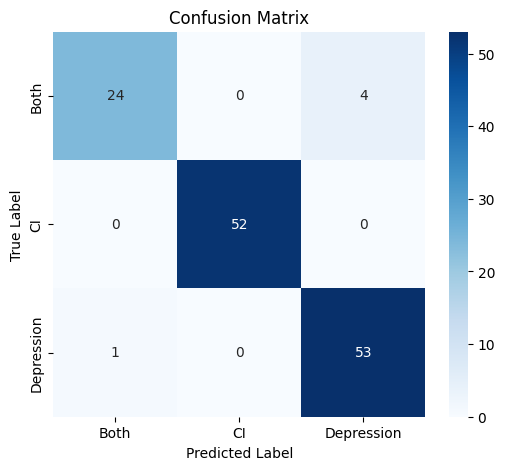
\includegraphics[width=0.6\textwidth]{confusion_matrix.png}
\caption{Confusion matrix of the Random Forest classifier}
\end{figure}

\section{Conclusion}

This study investigated the use of machine learning techniques to predict diagnostic outcomes based on patient demographic and clinical features. Through comprehensive exploratory data analysis, feature selection, and systematic model comparison, Random Forest was identified as the most effective algorithm.

The final model achieved strong predictive performance on unseen data, demonstrating that ensemble tree-based methods are well suited for structured healthcare datasets where nonlinear relationships and feature interactions are present.

Future work could explore additional ensemble techniques or larger datasets to further improve predictive performance.

\end{document}